\section{All-SAT Solver Using Backbone Techniques} \label{sec:meth}
We propose and implement an All-SAT solver \tool, which uses backbone information to get shorter partial solutions comparing to other tools.
With the help of shorter partial solutions, the number of SAT calls in \tool significantly reduces and the efficiency increases.

\subsection{Overview of Algorithms}
Figure \ref{fig:overflow} shows the workflow of \tool.
Given a formula $F$, \tool first computes the backbone variables of $F$ using tools from \cite{bb}.
For every backbone variable $bl$ of $F$, $bl\in \BL(F)$, and $bl$ is added to $F$ as a unit clause. During the computation of backbone variables, solutions are also generated and stored in $S(F)$. The partial solution of each solution $v\in S(F)$ is stored in $P(F)$.
\tool then computes the partial solution $p=partial(v)$ and the blocking clause $C$ for every solution in $S(F)$, and adds the partial solutions to $P(F)$. 
All backbone variables are removed from the partial solution $p$ of a solution $v$, and every essential but non-backbone literal remains in $p$. If every clause is satisfied with the current $p$, i.e., $\forall c\in F, p(c)=1$, the generation of $p$ completes, otherwise, more literals are added to $p$ based on a greedy strategy.
The blocking clause $C$ of a partial solution $p$ is the negation of $p$. For example, if $p=a\wedge b \wedge c$, then the blocking clause $C$ of $p$ is $C=\neg a \vee \neg b \vee \neg c$.
After generating the blocking clause $C$, $F$ is updated with the conjunction between $F$ and $C$, i.e. $F=F\wedge C$.
If $F\wedge C$ is unsatisfiable, then \tool has found every solution of the formula $F$.
Otherwise, a new solution $v'$ is returned by the SAT solver, \tool then computes the partial solution $p'$ and the blocking clause $C'$ again and updates the formula $F$ with $F\wedge C'$.
The updating of the formula $F$ continues until $F$ is unsatisfiable.
\tool then adds every backbone variable in $\BL(F)$ to every partial solution, and every solution of the given formula $F$ is represented in at least one of the partial solution.


\begin{figure}
    \centering
    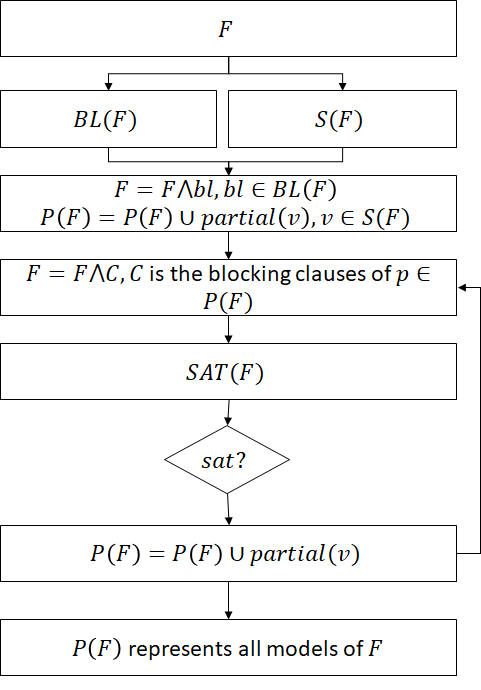
\includegraphics[scale=0.4]{workflow.png}
    \caption{Workflow of \tool}
    \label{fig:overflow}
\end{figure}

\subsection{Algorithms of \tool}
Algorithm \ref{alg:main} shows the main algorithm of \tool, where backbone($F$) uses the algorithms of backbone computing in~\cite{bb}.
The details of blocking($F$) are showed in Algorithm \ref{alg:pc}.
In Algorithm \ref{alg:main}, at Line \ref{ln:P}, the set of partial solutions and blocking clauses are initialized with $\emptyset$. The backbone variables of $F$ is computed, stored in $\BL(F)$ and added to $F$ as unit clauses. The solutions obtained from the backbone computation are stored in $S(F)$.
For every solution $v\in S(F)$, the partial solution $p$ and the blocking clause $C$ are computed and stored in $P(F)$ and $BC(F)$ respectively. 
At Line \ref{ln:bc}, the blocking clauses in $BC(F)$ are added to $F$, $ret$ is assigned with the satisfiability of $F$, returned by the Minisat Solver. If $F$ is satisfiable, then $v$ is a new solution of $F$, the partial solution $p$ and the blocking clause $C$ of the new solution $v$ is computed at Line \ref{ln:cvt}, and $F$ is updated with $F\wedge C$ again. The while loop at Line \ref{ln:check} continues if $F$ is satisfiable, otherwise \tool finishes the computing of every solution for the input formula, which is represented by at least one of the partial solutions in $P(F)$.

\begin{algorithm}
\SetKwInOut{Input}{Input}
\SetKwInOut{Output}{Output}
\SetAlgoShortEnd
\SetFillComment
\Input{A formula $F$}
\Output{Every satisfiable assignments of $F$}
$P(F):=\emptyset$\; \label{ln:P}
$BC(F):=\emptyset$\; \label{ln:BC}
$\BL(F),S(F):=backbone(F)$\; \label{ln:bl}
$F:=F\bigwedge bl, bl\in \BL(F)$\; \label{ln:u}
\ForEach {$v\in S(F)$}{ \label{ln:vt}
	$p,C:=blocking(v)$\; \label{ln:vb}
	$P(F):=P(F)\cup p$\; \label{ln:vp}
	$BC(F):=BC(F)\cup C$\; \label{ln:vbc}
}
$F:=F\bigwedge C, C\in BC(F)$\; \label{ln:bc}
$(ret, v) := SAT(F)$\; \label{ln:check}
\While {ret}{ \label{ln:check-true}
	$p,C:=blocking(v)$\; \label{ln:cvt}
	$P(F):=P(F)\cup p$\; \label{ln:cvb}
	$BC(F):=BC(F)\cup C$\; \label{ln:cvp}
	$F:=F\wedge C$\; \label{ln:cbc}
	$(ret,v):=SAT(F)$\; \label{ln:dc}
}
\Return $P(F)$\; \label{ln:ps}
\caption{Main Algorithm of \tool}\label{alg:main}
\end{algorithm}

In Algorithm \ref{alg:pc}, the partial solutions and the blocking clauses are computed. 
The input of Algorithm \ref{alg:pc} is a formula $F$, the backbone variables $\BL(F)$ of the given formula $F$ and a full solution $v$ returned by the Minisat Solver.
The partial solution $p$ and the blocking clause $C$ of $v$ are initialized as $\emptyset$ at Line \ref{ln:init}.
For every literal $l$ in $v$ such that $v(l)=1$, the algorithm first checks that if $x(l)$ is a backbone variable at Line \ref{ln:check-bl}. If $x(l)$ is a backbone variable, then $l$ is not added to $p$ at this step. Otherwise, $l$ is added to $p$ if there exists a clause $c$ such that $l$ is an essential variable with the given solution $v$ ( $l$ is the only literal in $c$ assigns to $1$ in $v$, from Line \ref{ln:us} to Line \ref{ln:ue}). $\neg l$ is added to the blocking clause $C$ if $l$ is added to the partial solution $p$. 
Starting from Line \ref{ln:cov}, the algorithm checks if every clause $c\in F$ is satisfied by the $p$, i.e., for every clause $c\in F$, there exists at least one literal $l\in c$, and $p(l)=1$. If a clause $c$ is not satisfied by the partial solution $p$, and there does not exist a backbone variable $bl\in c$, $v(bl)=1$, then a literal $l\in c, v(l)=1$ is added to $p$, and the literal $\neg l$ is added to $C$. 
In order to make $p$ a partial solution (instead of a partial assignment) of $v$, all backbone variables are added to $p$ at Line \ref{ln:bl}, but the blocking clauses remain the same since the backbone variables are already added to $F$ as unit clauses.
After executing the loop starting from Line \ref{ln:cov} and the adding of backbone variables at Line \ref{ln:bl}, every clause in $F$ is satisfied by the partial solution $p$, $p$ and $C$ are then returned by Algorithm \ref{alg:pc}.
\begin{algorithm}
\SetKwInOut{Input}{Input}
\SetKwInOut{Output}{Output}
\SetAlgoShortEnd
\SetFillComment
\Input{A formula $F$, a full solution $v\models F$ returned by Minisat Solver, the backbone variables $\BL(F)$ of $F$}
\Output{the partial solution $p$ and the blocking clauses $C$ of $v$}
$p:=\emptyset$\;
$C:=\emptyset$\; \label{ln:init}
\ForEach {$l\in v$}{
	\If {$x(l)\in \BL(F)$}{ continue\;} \label{ln:check-bl}
	\If {$\exists c\in F, l\in c$}{
		unique:=true\; \label{ln:us}
		\ForEach {$l'\neq l, l'\in c$}{
			\If {$v(l')=$}{
				unique:=false\;
				break\;
			}
		}
		\If {unique}{ \label{ln:ue}
			$p:=l\wedge l$\;
			$C:=C\vee \neg l$\;
		}
	}
}
\ForEach {$c\in F, (\not\exists bl\in c, bl\in \BL(F))\wedge(\not\exists l\in p, l\in c)$}{ \label{ln:cov}
	\ForEach {$l'\in c$}{
		$p:=l'\wedge l'$\;
		$C:=C \vee \neg l'$\;
		break\;
	}
}
\ForEach {$bl\in \BL(F)$}{ \label{ln:bl}
	$p:=p\wedge bl$\;
}
\Return $p, C$\;
\caption{Computing the Partial Solutions and the Blocking Clauses}\label{alg:pc}
\end{algorithm}

\begin{theorem} \label{theo:bl}
For a backbone variable $bl$ of a given formula $F$, if a partial solution $p\models F$, then $bl$ is in $p$ and $p(bl)=1$.
\end{theorem}

\begin{proof}
Given a formula $F$ and a backbone variable $bl$ of $F$, suppose there exists a partial solution $p$ such that $p(bl)=$ NOT\_KNOWN. Then there must exist two different solutions of $F$, such that for every variable $x\neq bl$, $v_1(x)=v_2(x)=v(x)$, and $v_1(bl)=\neg v_2(bl)=1$ or $v_1(bl)=\neg v_2(bl)=0$. In both cases, $bl$ is not a backbone variable of $F$ which contradicts with the assumptions that $bl$ is a variable of $F$.
\end{proof}
According to Theorem \ref{theo:bl}, there does not exist a partial solution $p$ such that a backbone variable $bl$ is not in $p$. Therefore, it is correct and essential to add all backbone variables back to every partial solution.

The main contribution of \tool is to use backbone variables in the computing of partial solutions and the blocking clauses. As proved in Theorem \ref{theo:bl}, every backbone variable must appear in every partial solution. Therefore, \tool removes the backbone variables and generates blocking clauses without them in it. To simplify the following SAT solving, backbone variables are used as initial assumptions by adding them back as unit clauses. With shorter blocking clauses, the complexity of the following SAT solving decreases. \tool is more efficient when the number of backbone variables in the formulas are larger. 

With the help of backbone variables, for some of the formulas, All-SAT computing terminates without any blocking clauses.
For a given formula $F$, whenever every clause $c\in F$ is satisfied by at least one backbone literal of $F$, \tool terminates. Since the set of backbones is the only one partial solution that represents every full solution of $F$.

Given a formula $F=(a\vee b)\wedge(a \vee \neg b)\wedge (\neg a \vee c \vee \neg d)$.
Table \ref{tab:comp} shows the All-SAT computing procedure of $F$.
\tool first computes the backbone variables of $F$, $a$ is the backbone variable of $F$, and the solution found during the backbone computing is $v=a\wedge b\wedge c \wedge d$. The partial solution $p$ and the blocking clause $C$ returned by Algorithm \ref{alg:pc} are $p=c$ and $C=\neg c$, respectively. 
Then $F$ is updated with the backbone variables and the blocking clauses, the backbone variable $a$ is added to $F$ as unit clause, and the blocking clause $\neg c$ is also added to $F$. The updated $F$ is $F=(a\vee b)\wedge(a \vee \neg b)\wedge (\neg a \vee c \vee \neg d)\wedge a\wedge \neg c$.
A new solution $v'=a\wedge b\wedge \neg c \wedge \neg d$ for the formula $F$ is computed. $p=\neg d$ and $C=d$ are returned by Algorithm \ref{alg:pc}.
Then $F$ is updated with $F=(a\vee b)\wedge(a \vee \neg b)\wedge (\neg a \vee c \vee \neg d)\wedge a\wedge \neg c\wedge d$. $F$ is unsatisfiable, and the All-SAT computing of $F=(a\vee b)\wedge(a \vee \neg b)\wedge (\neg a \vee c \vee \neg d)$ finished.
The solutions of $F=(a\vee b)\wedge(a \vee \neg b)\wedge (\neg a \vee c \vee \neg d)$ are represented with either $a\wedge \neg c$ or $a\wedge d$.

\begin{table*}
\begin{tabular}{ccccc}
\toprule
Formula & Full Solution & Backbone Variables & Partial Solution & Blocking Clauses \\
\midrule
$(a\vee b)\wedge(a \vee \neg b)\wedge (\neg a \vee c \vee \neg d)$ & $a\wedge b\wedge c\wedge d$ & $a$ & $c$ & $\neg c$ \\
$(a\vee b)\wedge(a \vee \neg b)\wedge (\neg a \vee c \vee \neg d)\wedge a\wedge \neg c$ &  $a\wedge b\wedge c\wedge d$ & $a$ & $\neg d$ & $d$ \\
$(a\vee b)\wedge(a \vee \neg b)\wedge (\neg a \vee c \vee \neg d)\wedge a\wedge \neg c\wedge d$ & Unsatisfiable &  & & \\
\bottomrule
\end{tabular}
    \caption{Computing Procedure of \tool }
    \label{tab:comp}
\end{table*} 


